% Options for packages loaded elsewhere
\PassOptionsToPackage{unicode}{hyperref}
\PassOptionsToPackage{hyphens}{url}
\documentclass[
]{article}
\usepackage{xcolor}
\usepackage{amsmath,amssymb}
\setcounter{secnumdepth}{-\maxdimen} % remove section numbering
\usepackage{iftex}
\ifPDFTeX
  \usepackage[T1]{fontenc}
  \usepackage[utf8]{inputenc}
  \usepackage{textcomp} % provide euro and other symbols
\else % if luatex or xetex
  \usepackage{unicode-math} % this also loads fontspec
  \defaultfontfeatures{Scale=MatchLowercase}
  \defaultfontfeatures[\rmfamily]{Ligatures=TeX,Scale=1}
\fi
\usepackage{lmodern}
\ifPDFTeX\else
  % xetex/luatex font selection
\fi
% Use upquote if available, for straight quotes in verbatim environments
\IfFileExists{upquote.sty}{\usepackage{upquote}}{}
\IfFileExists{microtype.sty}{% use microtype if available
  \usepackage[]{microtype}
  \UseMicrotypeSet[protrusion]{basicmath} % disable protrusion for tt fonts
}{}
\makeatletter
\@ifundefined{KOMAClassName}{% if non-KOMA class
  \IfFileExists{parskip.sty}{%
    \usepackage{parskip}
  }{% else
    \setlength{\parindent}{0pt}
    \setlength{\parskip}{6pt plus 2pt minus 1pt}}
}{% if KOMA class
  \KOMAoptions{parskip=half}}
\makeatother
\usepackage{graphicx}
\makeatletter
\newsavebox\pandoc@box
\newcommand*\pandocbounded[1]{% scales image to fit in text height/width
  \sbox\pandoc@box{#1}%
  \Gscale@div\@tempa{\textheight}{\dimexpr\ht\pandoc@box+\dp\pandoc@box\relax}%
  \Gscale@div\@tempb{\linewidth}{\wd\pandoc@box}%
  \ifdim\@tempb\p@<\@tempa\p@\let\@tempa\@tempb\fi% select the smaller of both
  \ifdim\@tempa\p@<\p@\scalebox{\@tempa}{\usebox\pandoc@box}%
  \else\usebox{\pandoc@box}%
  \fi%
}
% Set default figure placement to htbp
\def\fps@figure{htbp}
\makeatother
\setlength{\emergencystretch}{3em} % prevent overfull lines
\providecommand{\tightlist}{%
  \setlength{\itemsep}{0pt}\setlength{\parskip}{0pt}}
\usepackage{bookmark}
\IfFileExists{xurl.sty}{\usepackage{xurl}}{} % add URL line breaks if available
\urlstyle{same}
\hypersetup{
  pdftitle={Posterior-Based Decision Stability in Urban Flood Risk Prioritisation},
  hidelinks,
  pdfcreator={LaTeX via pandoc}}

\title{Posterior-Based Decision Stability in Urban Flood Risk
Prioritisation}
\author{Mikel Martinez Mugica\\
Independent Researcher\\
https://habnetic.org}
\date{March 2026}

\begin{document}
\maketitle

\section{Abstract}\label{abstract}

This project investigates the stability of prioritisation decisions in
urban pluvial flood risk assessments under epistemic uncertainty.
Existing approaches often quantify uncertainty within individual
components of the exposure--hazard--impact chain, but rarely propagate
it coherently to the prioritisation outputs that guide intervention.

The project proposes a unified hierarchical Bayesian framework linking
exposure, hazard, and impact within a single generative model. Rather
than focusing only on expected loss estimates, the framework derives
posterior distributions over prioritisation rankings. Decision-level
quantities such as rank distributions and top-(k) membership
probabilities are treated as primary inferential outputs.

The empirical reference case is Rotterdam, where a city-scale spatial
pipeline has already been developed for approximately 221,000 buildings.
The framework is further extended through cross-city transfer under a
fixed generative specification, interpreted as a structural stress test.

The project reframes urban pluvial risk modelling from expected-loss
estimation toward inference about the robustness of prioritisation
decisions under uncertainty.

\section{1. Introduction and Problem}\label{introduction-and-problem}

Urban flood risk assessments are routinely used to support
infrastructure investment and resilience planning. In practice, these
decisions often take the form of prioritisation: given limited
resources, which buildings, streets, or neighbourhoods should be
protected first?

A municipality may need to select a small subset of assets, for example
the 500 most critical buildings out of more than 200,000, for targeted
mitigation. This selection is usually based on rankings derived from
estimated risk or expected loss.

The difficulty is that such rankings are built on uncertain inputs.
Exposure, hazard, and impact are all modelled under incomplete data,
imperfect assumptions, and epistemic uncertainty. Yet in many practical
workflows this uncertainty is reduced to point estimates and then
converted into a single deterministic ranking.

In practice, this usually means estimating a risk value for each asset
and then sorting all assets from highest to lowest priority. In
simplified form, that decision step can be written as

\[
\operatorname{rank}_i = \operatorname{argsort}\!\left(\mathbb{E}[\operatorname{risk}_i]\right)
\]

This creates a mismatch between modelling and decision-making.
Uncertainty is acknowledged within components of the model, but it
disappears at the very step where intervention priorities are derived.
As a result, it remains unclear whether prioritisation outcomes are
robust or whether small changes in assumptions could lead to different
decisions.

This project addresses that gap by treating prioritisation itself as an
uncertain quantity. Instead of producing one ranking, it derives a
distribution over rankings from a joint posterior distribution.

The central research question is therefore:

\begin{quote}
\textbf{How stable are prioritisation decisions in urban pluvial risk
assessments once uncertainty is propagated coherently across the full
exposure--hazard--impact chain?}
\end{quote}

In simple terms: if two assets are ranked near the decision boundary,
are we looking at a robust priority or at a hidden coin toss?

\section{2. Literature Review and
Positioning}\label{literature-review-and-positioning}

Research on uncertainty in flood risk assessment is substantial, but it
is spread across several partially disconnected strands.

A first strand consists of \textbf{Bayesian damage models}, such as
Sairam et al.~(2019), Mohor et al.~(2021), and Lv et al.~(2021). These
studies show that hierarchical Bayesian approaches are effective for
modelling flood damage under sparse and heterogeneous data conditions.
However, their inferential targets remain parameter estimation,
predictive performance, and transferability of impact models.
Prioritisation is still usually derived from expected losses or summary
statistics.

A second strand focuses on \textbf{end-to-end physical uncertainty
propagation}, for example McMillan and Brasington (2008). This work
recognises that uncertainty accumulates across hydrological and
hydraulic model cascades. Yet the main focus remains physical process
representation, and the final prioritisation step is typically performed
outside the probabilistic framework.

A third strand uses \textbf{Bayesian networks and susceptibility
models}, such as Wu et al.~(2019, 2020), to produce probabilistic risk
maps from heterogeneous variables. These approaches are useful for
integrating multiple factors, but they do not derive posterior
distributions over asset-level prioritisation rankings within a
hierarchical exposure--hazard--impact structure.

A fourth strand includes \textbf{robust decision-making under deep
uncertainty}, such as Info-Gap and RDM (Hall \& Harvey, 2009; Matrosov
et al., 2013). This literature is highly relevant because it addresses
robustness explicitly. However, it generally operates on scenario
ensembles and policy alternatives rather than on posterior distributions
over ranking-based prioritisation outputs.

Taken together, these strands show that uncertainty is already
recognised as important in flood risk assessment. What remains missing
is not awareness of uncertainty itself, but a framework that carries it
coherently into the ranking outputs that directly support intervention
decisions. Across these strands, uncertainty is recognised, but the
final decision output is still rarely treated as the primary object of
probabilistic inference.

The present project sits at the intersection of these strands but makes
a different move. It does not propose a new hydraulic model, a new
damage function, or a new planning paradigm. Its contribution is to
connect exposure, hazard, and impact within a single probabilistic
framework and to treat prioritisation stability itself as the
inferential target.

\section{3. Research Gap and
Contribution}\label{research-gap-and-contribution}

The central gap lies at the interface between probabilistic modelling
and decision-making.

Existing work demonstrates how uncertainty can be represented: - within
model components, - across physical model chains, - or across planning
scenarios.

What remains largely missing is a framework that carries epistemic
uncertainty coherently into the final prioritisation outputs used for
intervention.

This project addresses that gap by redefining the inferential target.
Rather than treating expected loss as the main output, it treats
prioritisation decisions themselves as posterior quantities.

The main novelty therefore lies not in proposing a new hazard model, but
in shifting the inferential focus from modelled risk to the stability of
the prioritisation decisions derived from it.

The project makes three main contributions:

\begin{enumerate}
\def\labelenumi{\arabic{enumi}.}
\item
  \textbf{Unified probabilistic structure}\\
  It formalises exposure, hazard, and impact within a single
  hierarchical posterior.
\item
  \textbf{Decision as a posterior quantity}\\
  It derives rankings and top-(k) membership from posterior draws rather
  than from expected values alone.
\item
  \textbf{Transfer as structural stress test}\\
  It evaluates the same generative specification across cities and
  interprets changes in ranking stability as evidence of structural
  robustness or sensitivity.
\end{enumerate}

In short, the project is not about building a better flood map. It is
about determining how reliable the decisions based on such models
actually are.

\section{4. Methodological Framework}\label{methodological-framework}

The framework conceptualises urban pluvial risk as a probabilistic
system linking exposure, hazard, impact, and decision:

\[
\text{Exposure} \rightarrow \text{Hazard} \rightarrow \text{Impact} \rightarrow \text{Decision}
\]

At the asset level, the relevant quantities are: - exposure indicators
(X\_i), - hazard intensity (H\_i), - impact outcome (Y\_i).

The generative structure is

\[
H_i \sim p(H \mid X_i, \theta_H)
\]

\[
Y_i \sim p(Y \mid H_i, X_i, \theta_Y)
\]

where (\theta\_H) and (\theta\_Y) denote hazard and impact parameters.

Hazard is treated as a probabilistic input variable informed by
long-term precipitation patterns rather than as a fully resolved
hydrodynamic simulation. In the current empirical implementation, (H\_i)
is approximated by an observed precipitation-derived proxy. More complex
latent hazard modelling is reserved for later stages of the project.

Bayesian inference yields a joint posterior over plausible system
states:

\[
p(\theta_H, \theta_Y, H \mid \text{data})
\propto
p(Y \mid H, X, \theta_Y)\, p(H \mid X, \theta_H)\, p(\theta_H)\, p(\theta_Y)
\]

This is important because the same inferential structure generates both
predictive quantities and decision-level outputs.

In Phase 1, the impact model is specified as a simple logistic
regression with synthetic binary outcome:

\[
\text{logit}(p_i) = \alpha + \beta_E X_i + \beta_H H_i
\]

\[
Y_i \sim \text{Bernoulli}(p_i)
\]

with weakly informative priors:

\[
\alpha, \beta_E, \beta_H \sim \mathcal{N}(0, 2.5)
\]

This baseline model is intentionally modest. Its purpose is not
hydraulic completeness, but transparent end-to-end uncertainty
propagation.

\begin{figure}
\centering
\pandocbounded{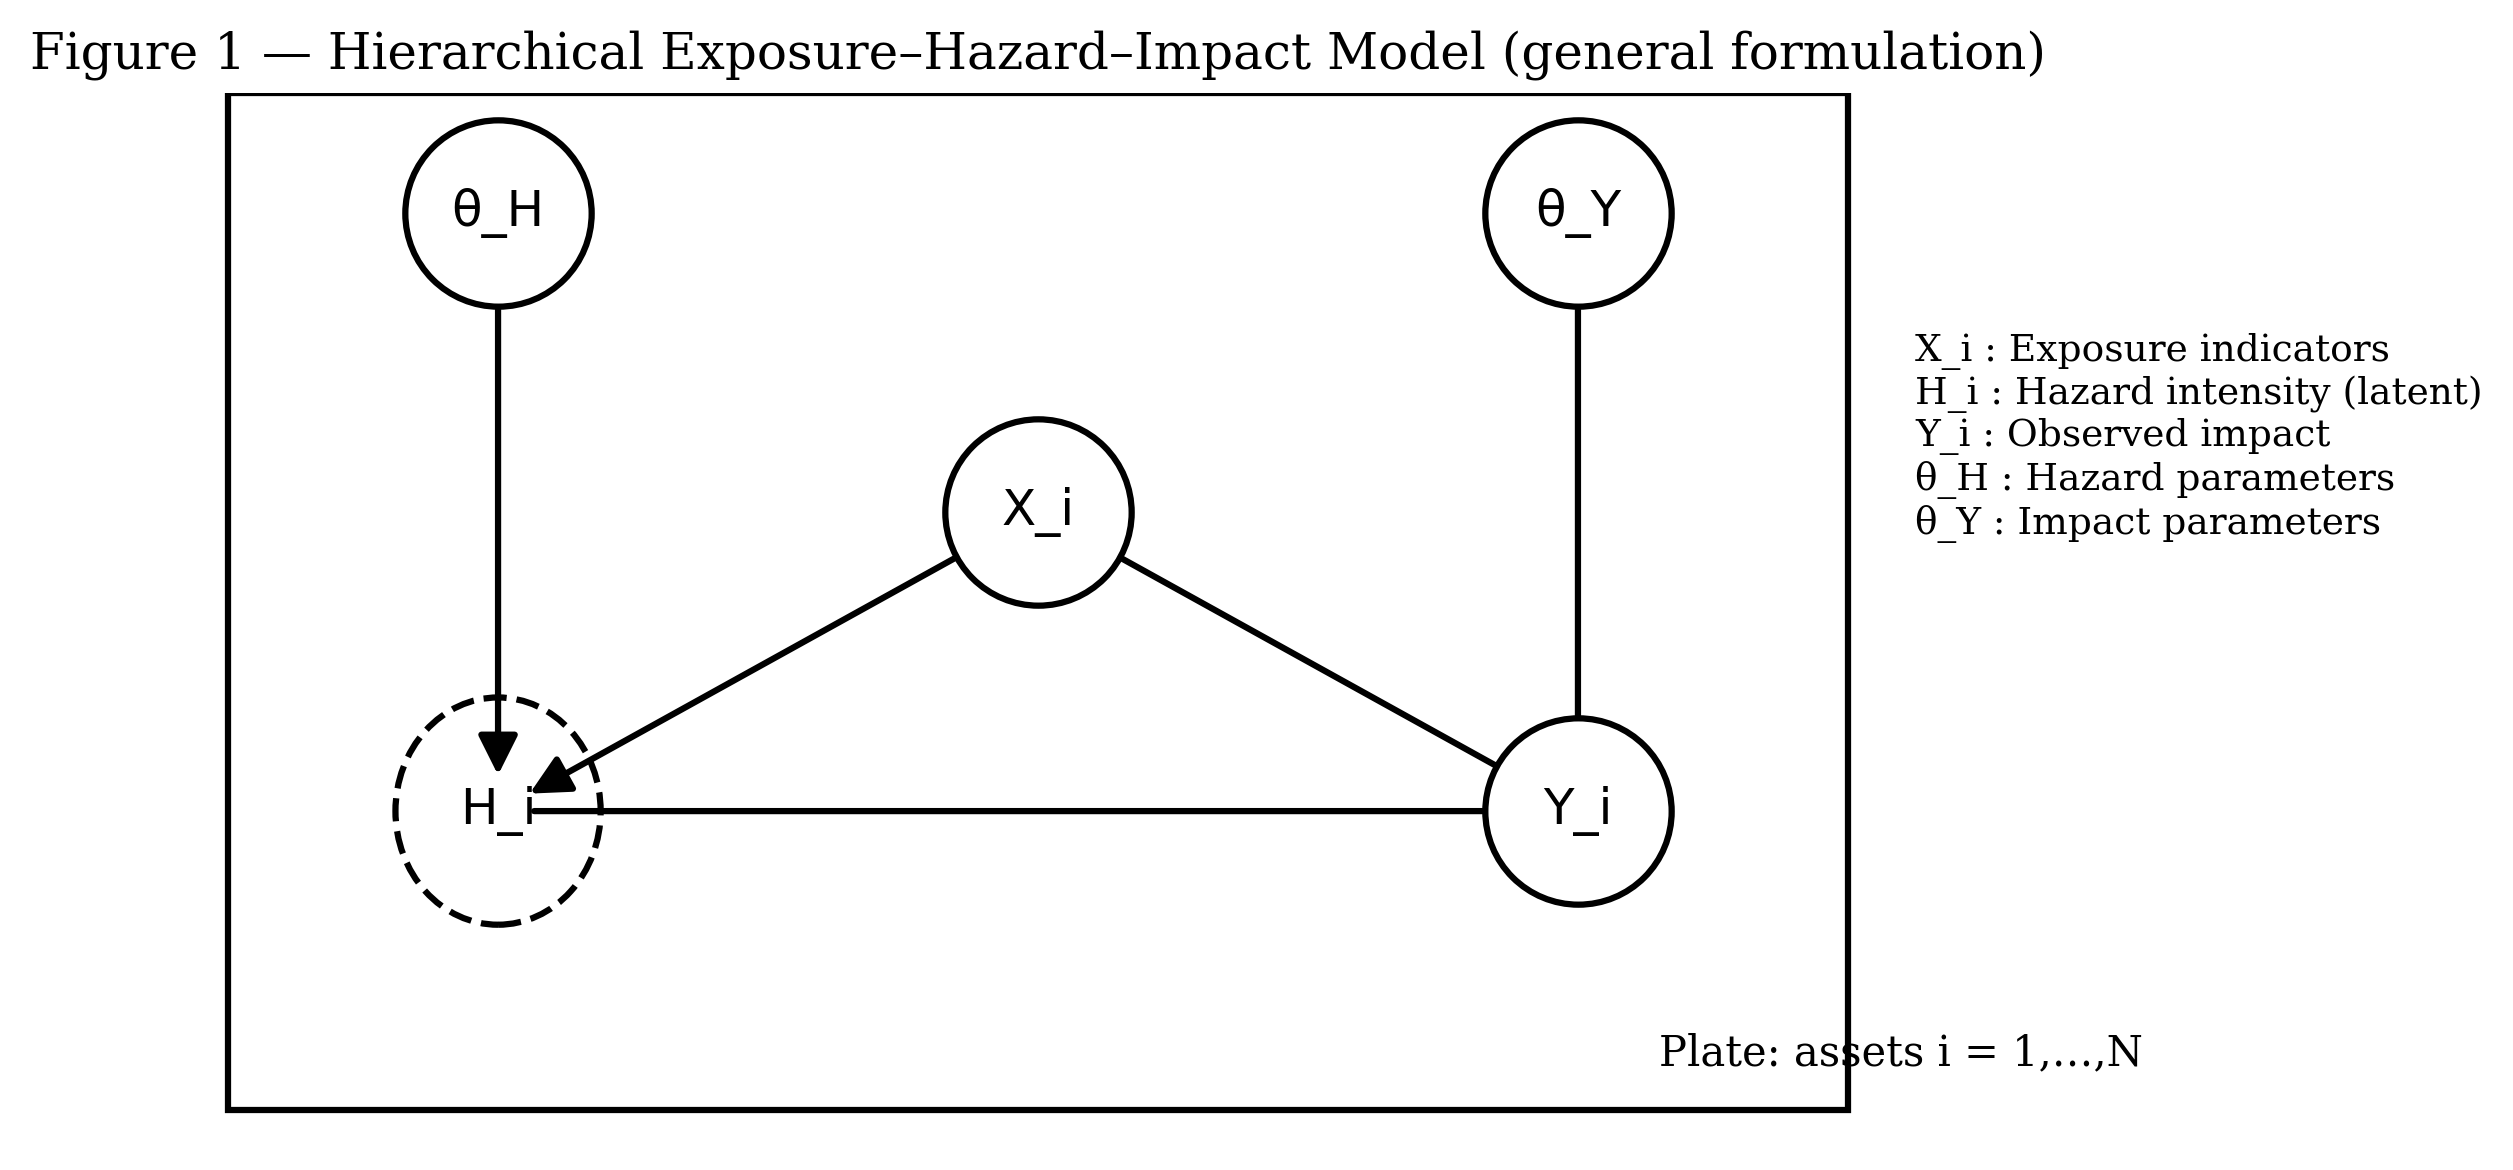
\includegraphics[keepaspectratio,alt={Hierarchical exposure--hazard--impact model}]{figures/fig01_graphical_model.png}}
\caption{Hierarchical exposure--hazard--impact model}
\end{figure}

\section{5. Decision-Level Inference}\label{decision-level-inference}

The central methodological shift occurs at the final step.

In conventional workflows, risk is estimated and then collapsed into a
single ranking. In the present framework, for each posterior draw (s),
asset-level risks are computed and converted into rankings:

\[
\text{rank}^{(s)} = \text{argsort}(\text{risk}^{(s)})
\]

This means prioritisation is represented not as one ordering, but as a
distribution over orderings.

The main decision-level quantities are:

\begin{itemize}
\tightlist
\item
  posterior rank distributions (r\_i\^{}\{(s)\}),
\item
  top-(k) membership probabilities,
\end{itemize}

\[
P(i \in \text{top-}k) = \frac{1}{S} \sum_{s=1}^{S} \mathbf{1}(i \in \text{top-}k^{(s)})
\]

\begin{itemize}
\tightlist
\item
  and ranking variability measures such as rank standard deviation.
\end{itemize}

These quantities allow a distinction between robust and unstable
priorities. If an asset appears in the top-(k) group in nearly every
posterior draw, its priority is stable. If it moves in and out of the
group depending on the draw, then it lies near a fragile decision
boundary.

In plain terms: instead of saying ``this building is ranked fifth,'' the
framework allows us to say ``this building is almost always among the
highest priorities'' or ``this building is only sometimes there.'' That
difference is exactly what matters when budgets force sharp decisions.

\begin{figure}
\centering
\pandocbounded{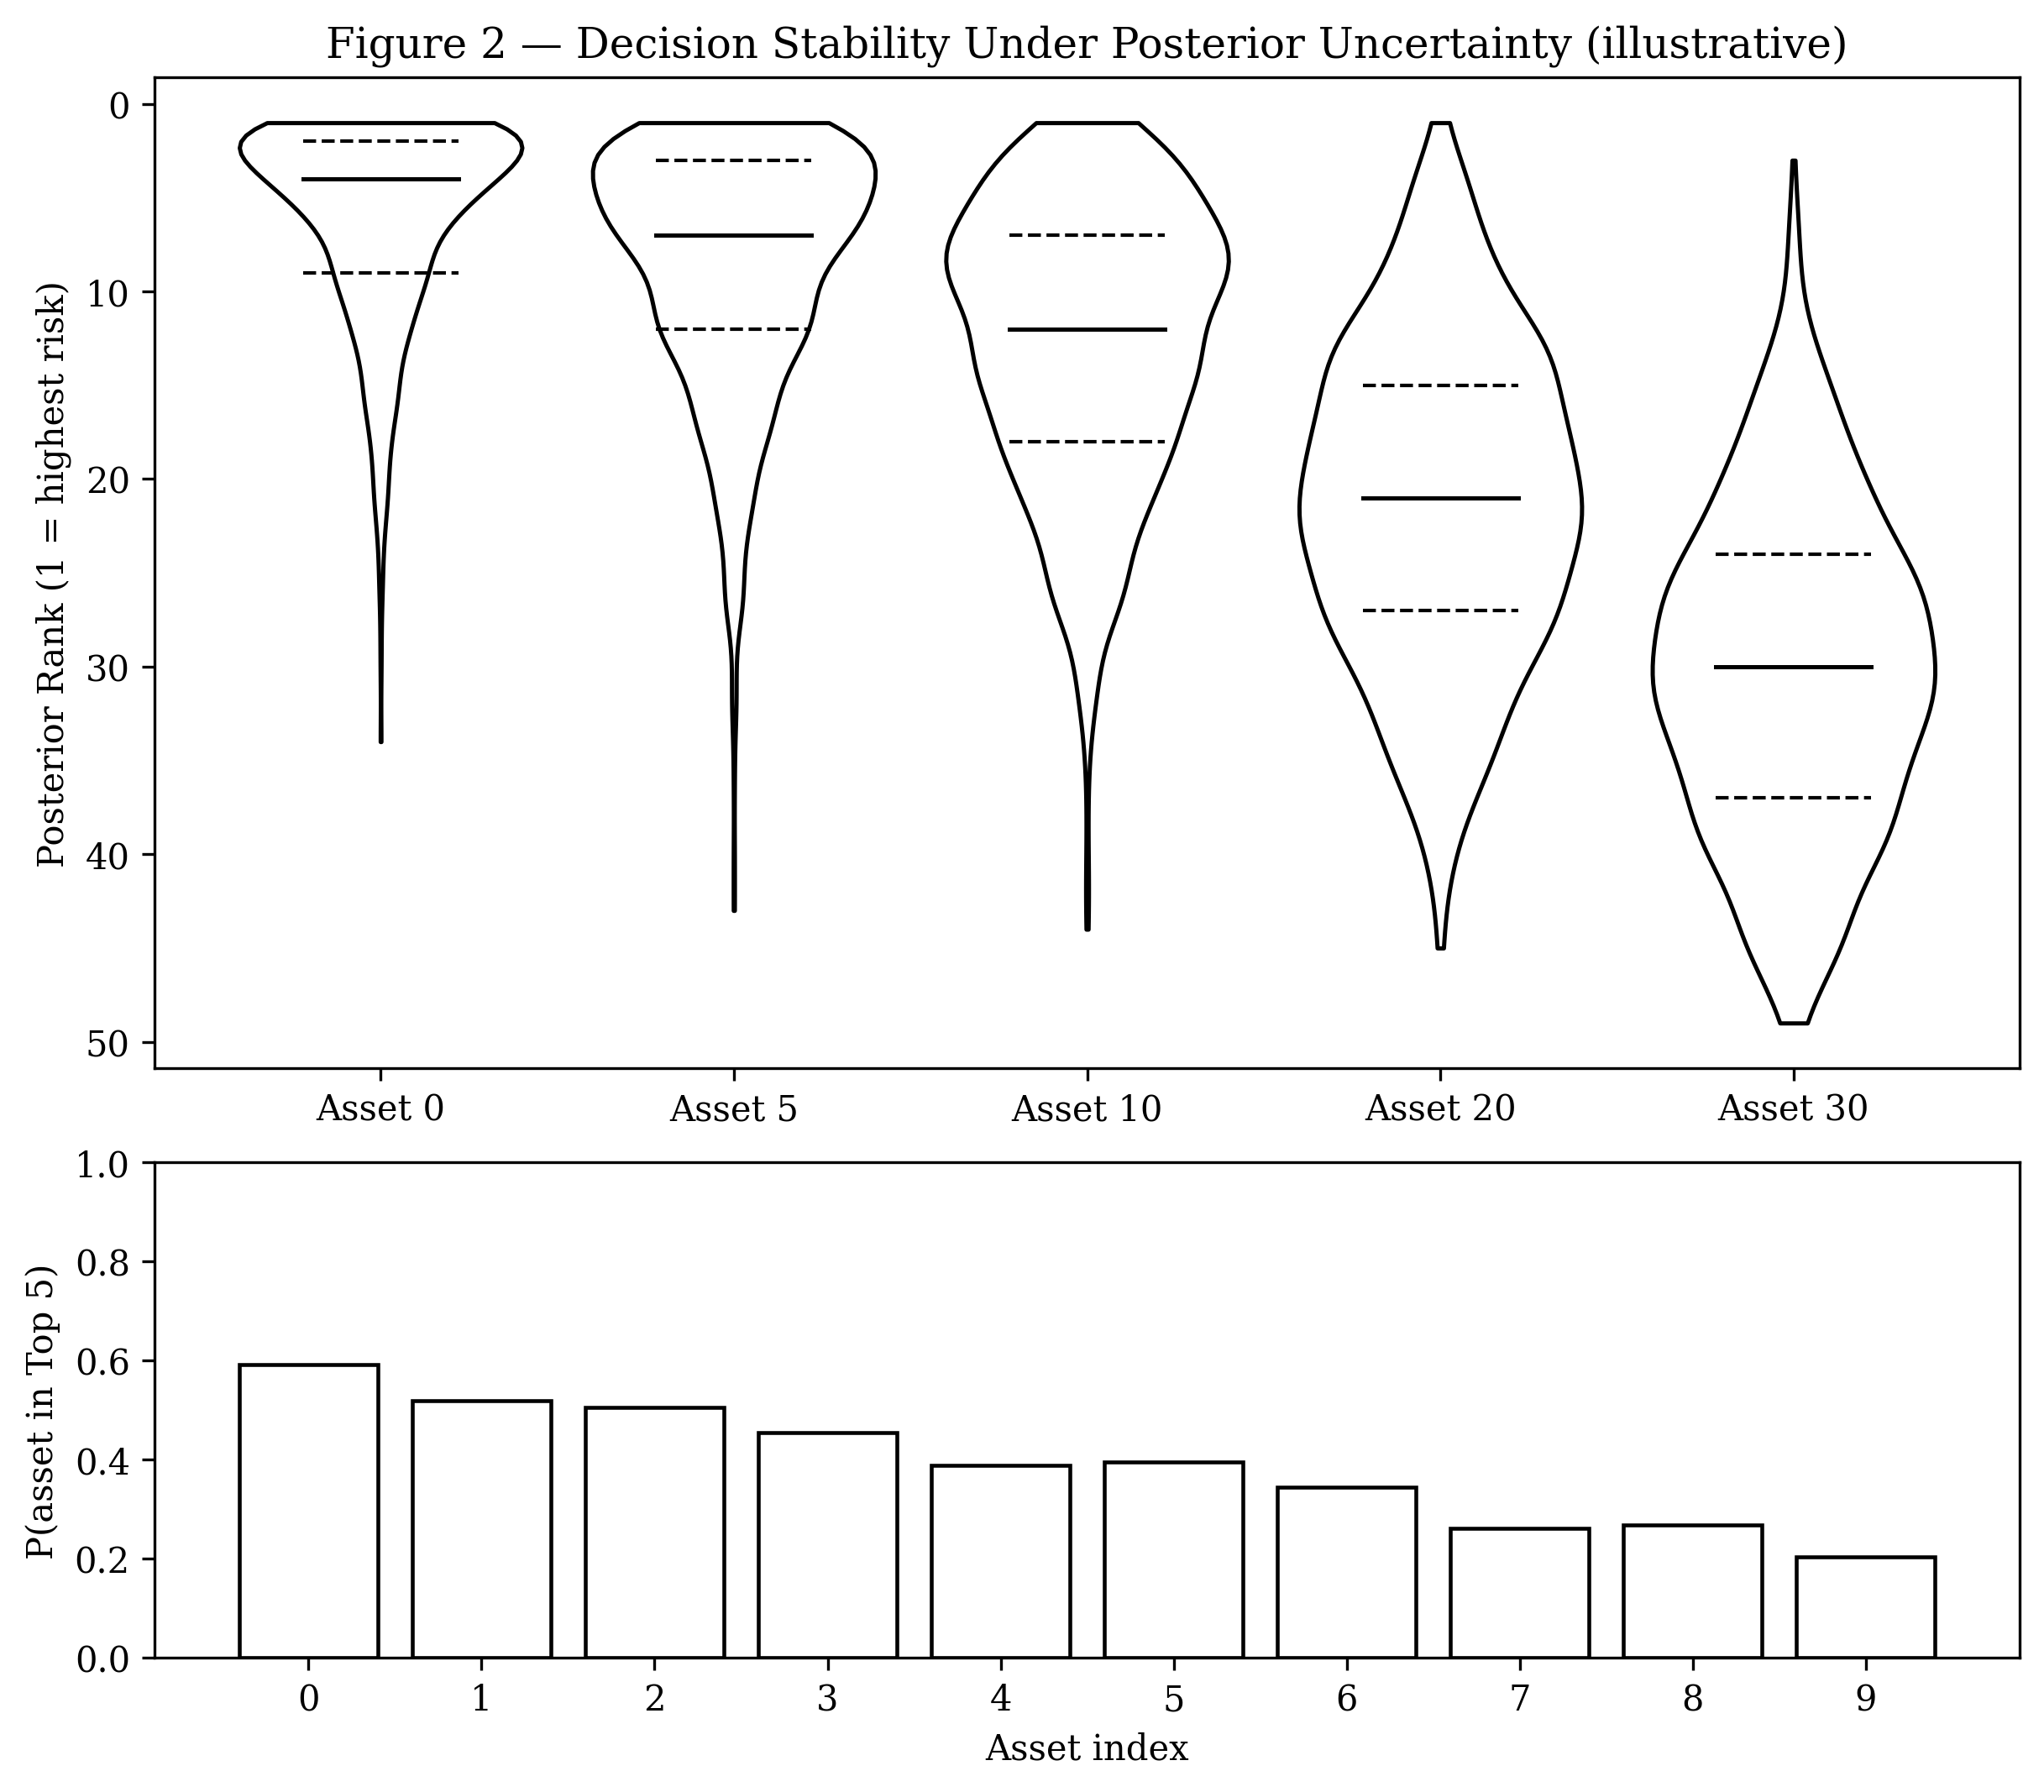
\includegraphics[keepaspectratio,alt={Decision stability concept}]{figures/fig02_decision_stability_concept.png}}
\caption{Decision stability concept}
\end{figure}

\section{6. Empirical Basis and Current
Progress}\label{empirical-basis-and-current-progress}

The empirical reference case is the municipality of Rotterdam, defined
using the CBS gebiedsindelingen 2025 administrative boundary and
comprising approximately 221,000 building footprints after clipping the
raw OpenStreetMap regional extract. A city-scale spatial data
integration pipeline has already been developed prior to the present
phase of modelling work.

The current dataset integrates: - building footprints from OpenStreetMap
regional extracts (via Geofabrik), - the authoritative Rotterdam
municipality boundary from CBS gebiedsindelingen 2025
(\texttt{gemeente\_niet\_gegeneraliseerd}), used as the spatial clip, -
hydrography layers, - ERA5-Land precipitation data, - exposure
indicators such as distance to water bodies and local hydrographic
density.

This work is important because the project does not begin from an
abstract idea alone. It already rests on an operational asset-level
pipeline at city scale.

The completed preparatory work includes: - reproducible spatial
preprocessing, - harmonisation of geospatial sources and identifiers, -
generation of building-level exposure indicators, - construction of a
precipitation-based hazard proxy, - implementation of an initial
Bayesian baseline model, - computation of preliminary decision-stability
metrics.

The current implementation uses a synthetic binary outcome variable and
a simplified hazard proxy. These simplifications are intentional. They
allow the project to validate the probabilistic inference and decision
pipeline before moving to richer hazard formulations and cross-city
transfer.

A first citywide output of the Phase 1 model is the distribution of
posterior mean impact probabilities across all buildings.

\begin{figure}
\centering
\pandocbounded{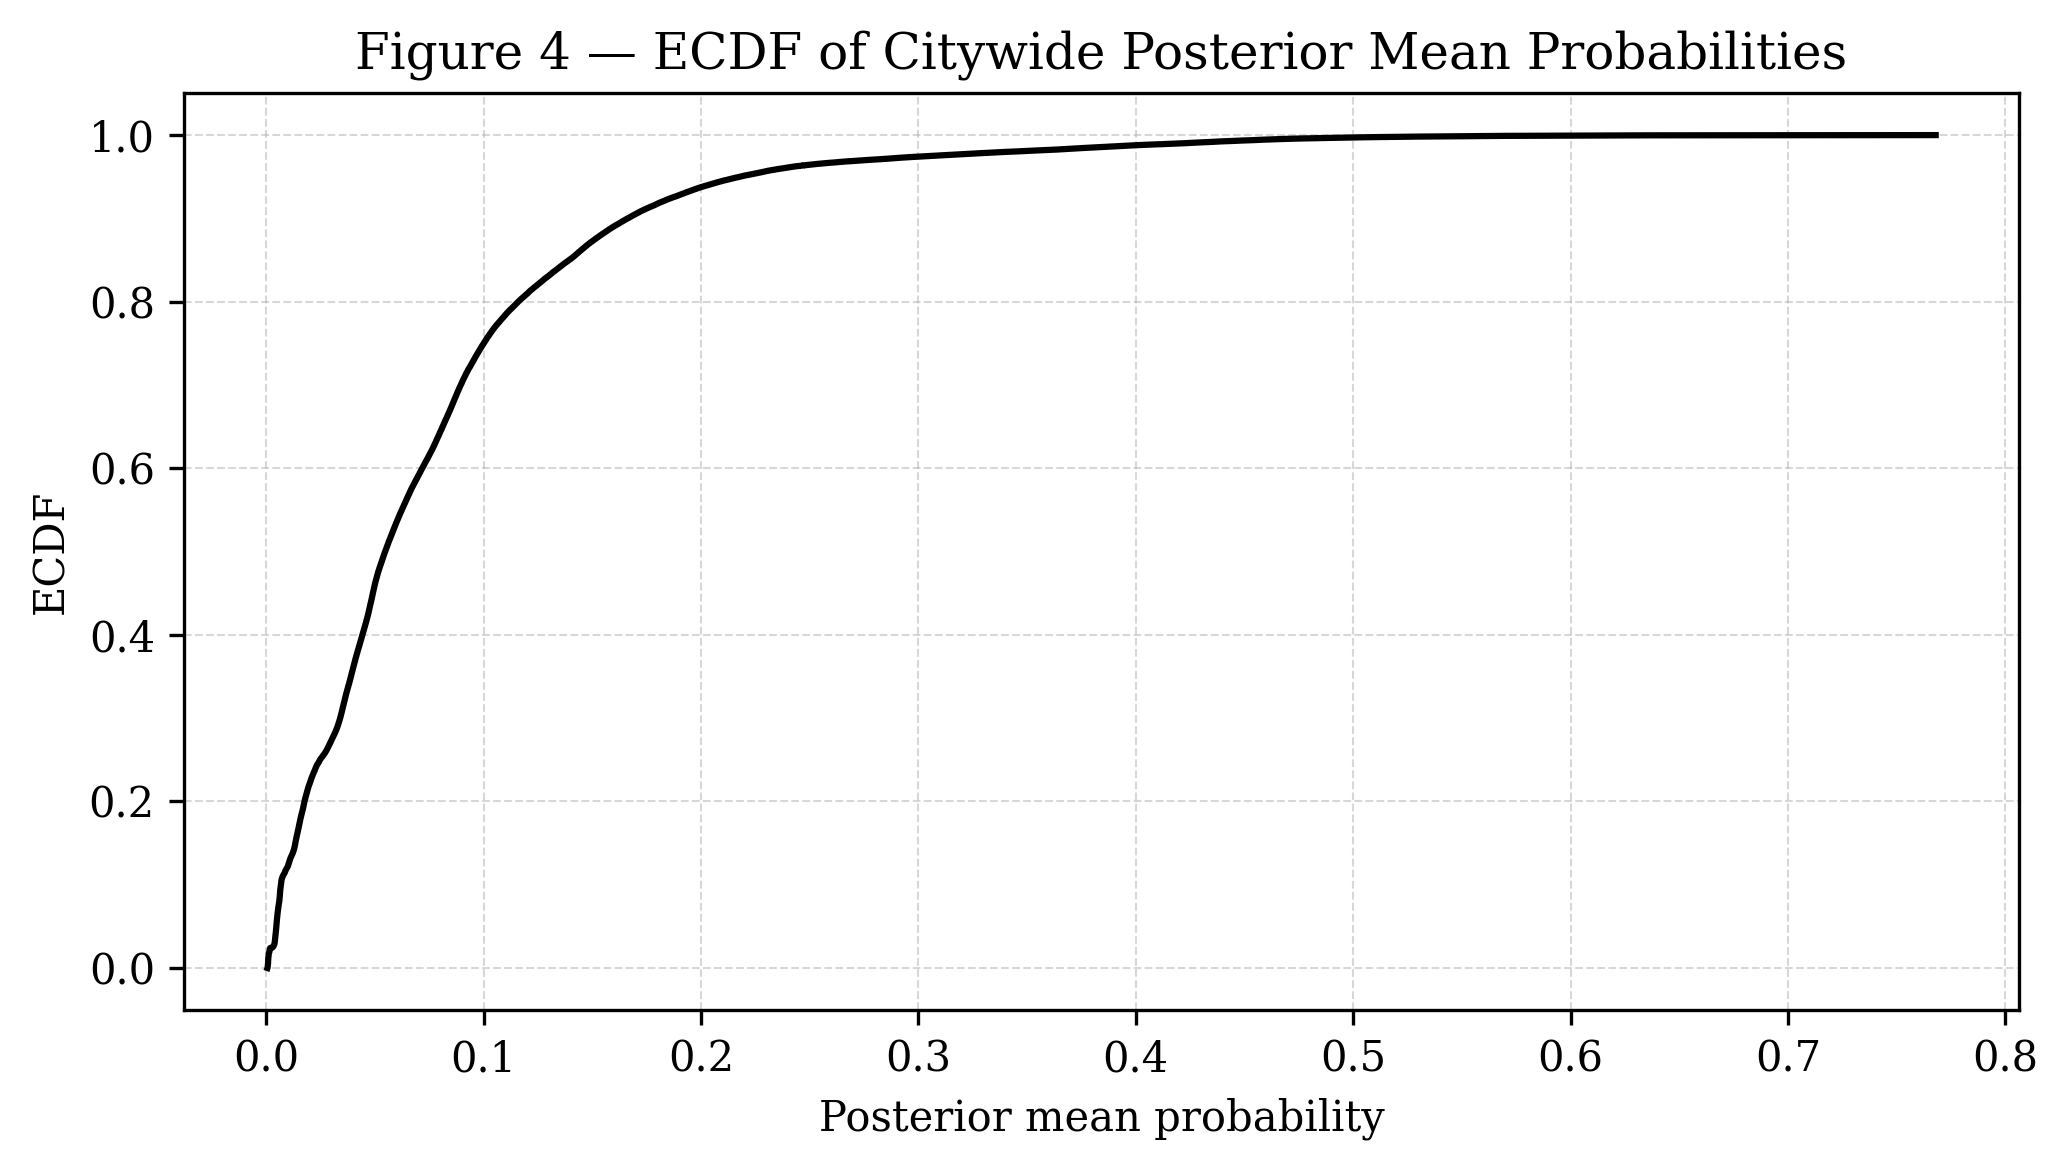
\includegraphics[keepaspectratio,alt={Empirical cumulative distribution of citywide posterior mean probabilities}]{figures/fig04_pmean_city_ecdf.png}}
\caption{Empirical cumulative distribution of citywide posterior mean
probabilities}
\end{figure}

Preliminary results already indicate that decision instability is
concentrated near relatively narrow prioritisation boundaries rather
than spread uniformly across the urban asset set.

\section{7. Cross-City Transfer and Work
Plan}\label{cross-city-transfer-and-work-plan}

A key part of the project is to apply the same model structure to
additional cities without redefining the generative specification.

This is not treated as recalibration. It is treated as a
\textbf{structural stress test}.

If ranking behaviour remains stable across contexts, that suggests the
framework captures relationships that generalise. If ranking variability
expands under transfer, that indicates sensitivity to contextual change
and therefore reveals limits of the modelling structure.

\begin{figure}
\centering
\pandocbounded{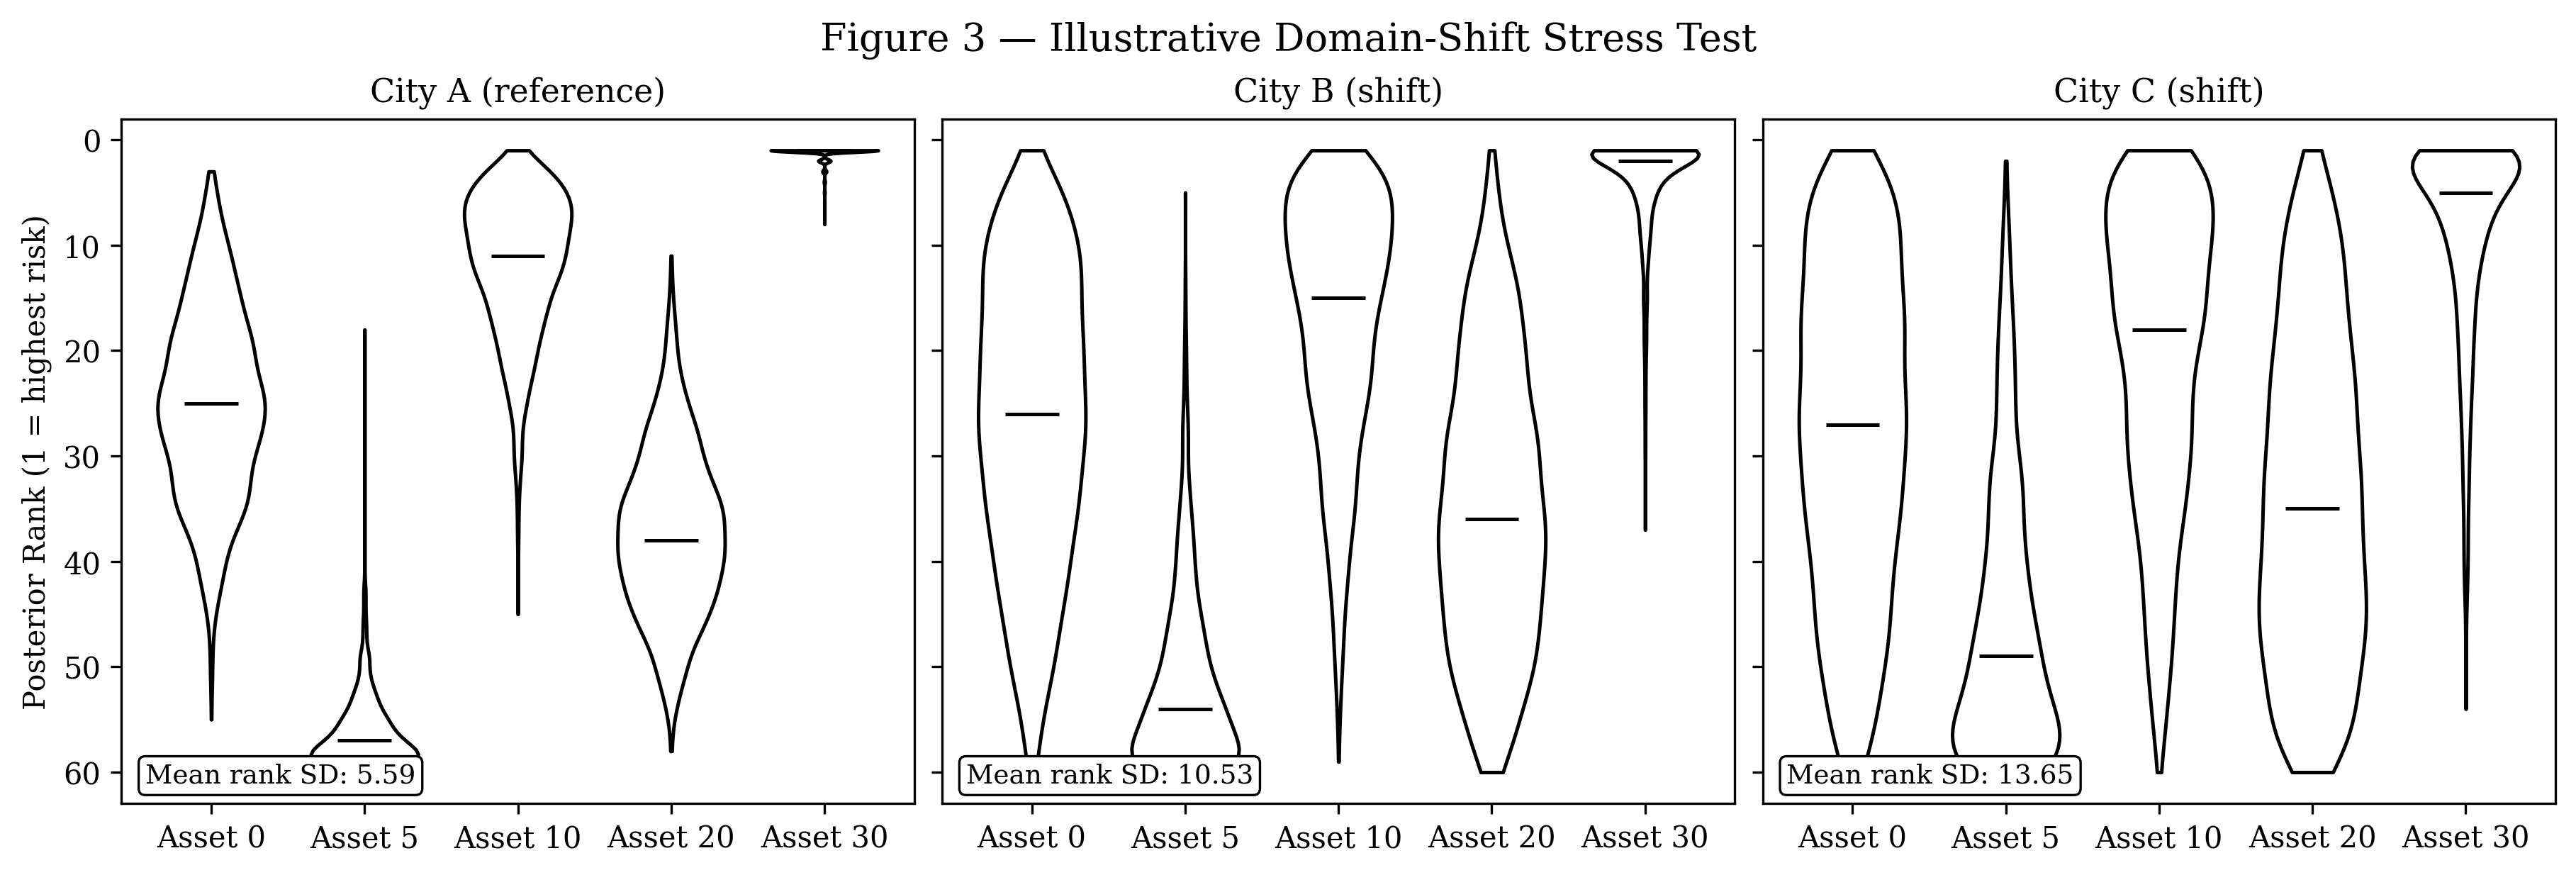
\includegraphics[keepaspectratio,alt={Domain-shift stress test concept}]{figures/fig03_domain_shift_illustrative.png}}
\caption{Domain-shift stress test concept}
\end{figure}

The project is organised in four phases from March 2026 to February
2027:

\subsection{Phase 1 --- Baseline probabilistic pipeline
(completed)}\label{phase-1-baseline-probabilistic-pipeline-completed}

\begin{itemize}
\tightlist
\item
  finalise Rotterdam dataset,
\item
  implement baseline Bayesian model,
\item
  compute posterior decision metrics,
\item
  prepare methodological working paper.
\end{itemize}

\subsection{Phase 2 --- Posterior decision stability
analysis}\label{phase-2-posterior-decision-stability-analysis}

\begin{itemize}
\tightlist
\item
  extend posterior analysis,
\item
  test prior and specification sensitivity,
\item
  evaluate alternative hazard proxies,
\item
  refine ranking stability measures.
\end{itemize}

\subsection{Phase 3 --- Cross-city structural
transfer}\label{phase-3-cross-city-structural-transfer}

\begin{itemize}
\tightlist
\item
  apply the fixed-specification model to additional cities,
\item
  analyse ranking behaviour under domain shift,
\item
  quantify instability changes across contexts.
\end{itemize}

\subsection{Phase 4 --- Model extension and
synthesis}\label{phase-4-model-extension-and-synthesis}

\begin{itemize}
\tightlist
\item
  introduce a latent hazard layer,
\item
  compare proxy-based and latent hazard formulations,
\item
  integrate findings across cities,
\item
  prepare journal manuscript.
\end{itemize}

\section{8. Expected Contributions and
Scope}\label{expected-contributions-and-scope}

The project is primarily methodological, with empirical work serving to
demonstrate the framework in practice.

Its main contributions are:

\begin{itemize}
\tightlist
\item
  formalisation of the exposure--hazard--impact chain within a unified
  hierarchical posterior;
\item
  treatment of prioritisation stability as an inferential target;
\item
  derivation of ranking distributions and top-(k) membership
  probabilities from posterior draws;
\item
  use of cross-city transfer as a diagnostic of structural robustness.
\end{itemize}

Empirically, the project is expected to: - quantify how epistemic
uncertainty affects prioritisation at city scale, - identify decision
boundaries where rankings are fragile, - and show how these behaviours
change under transfer.

The current phase has clear limits. Hazard is represented through a
precipitation proxy rather than a hydrodynamic model. The outcome
variable is synthetic and not calibrated against observed damage.
Exposure is represented through a limited set of hydrography-based
indicators. The results should therefore be interpreted as evidence
about the behaviour of the probabilistic framework rather than as
operational flood risk estimates.

Even with these limits, the project makes a clear shift:

\begin{quote}
from asking only ``what is the estimated risk?'' to asking ``how
reliable are the decisions based on that estimate?''
\end{quote}

\section{References}\label{references}

Gelman, A., Carlin, J. B., Stern, H. S., Dunson, D. B., Vehtari, A., \&
Rubin, D. B. (2013). \emph{Bayesian data analysis} (3rd ed.). CRC Press.

Hall, J. W., \& Harvey, H. (2009). Decision making under severe
uncertainties for flood risk management: A case study of Info-Gap
robustness analysis. In \emph{Proceedings of the 8th International
Conference on Hydroinformatics}, Concepción, Chile.

Lv, H., Wu, Z., Guan, X., \& Meng, Y. (2021). The construction of flood
loss ratio function in cities lacking loss data based on dynamic
proportional substitution and hierarchical Bayesian model. \emph{Journal
of Hydrology, 592}, 125797.
https://doi.org/10.1016/j.jhydrol.2020.125797

Matrosov, E. S., Woods, A. M., \& Harou, J. J. (2013). Robust decision
making and Info-Gap decision theory for water resource system planning.
\emph{Journal of Hydrology, 494}, 43--58.
https://doi.org/10.1016/j.jhydrol.2013.03.006

McElreath, R. (2020). \emph{Statistical rethinking: A Bayesian course
with examples in R and Stan} (2nd ed.). Chapman and Hall/CRC.

McMillan, H. K., \& Brasington, J. (2008). End-to-end flood risk
assessment: A coupled model cascade with uncertainty estimation.
\emph{Water Resources Research, 44}(3).
https://doi.org/10.1029/2007WR005995

Mohor, G. S., Thieken, A. H., \& Korup, O. (2021). Residential flood
loss estimated from Bayesian multilevel models. \emph{Natural Hazards
and Earth System Sciences, 21}, 1599--1614.
https://doi.org/10.5194/nhess-21-1599-2021

Raiffa, H., \& Schlaifer, R. (1961). \emph{Applied statistical decision
theory}. Harvard University Press.

Sairam, N., Schröter, K., Rözer, V., Merz, B., \& Kreibich, H. (2019). A
Bayesian hierarchical model for flood damage estimation in data-scarce
regions. \emph{Water Resources Research, 55}(11), 9129--9151.
https://doi.org/10.1029/2019WR025068

Vehtari, A., Gelman, A., \& Gabry, J. (2017). Practical Bayesian model
evaluation using leave-one-out cross-validation and WAIC.
\emph{Statistics and Computing, 27}, 1413--1432.
https://doi.org/10.1007/s11222-016-9696-4

Wu, Z., Shen, Y., Wang, H., \& Wu, M. (2019). Assessing urban flood
disaster risk using Bayesian network model and GIS applications.
\emph{International Journal of River Basin Management, 17}(4),
2163--2184. https://doi.org/10.1080/19475705.2019.1685010

Wu, Z., Shen, Y., Wang, H., \& Wu, M. (2020). Urban flood disaster risk
evaluation based on ontology and Bayesian network. \emph{Journal of
Hydrology, 583}, 124596. https://doi.org/10.1016/j.jhydrol.2020.124596

\end{document}
